\chapter{Algoritmus z bakalárskej práce}

V tejto práci naväzujeme a ďalej vylepšujeme algoritmus, ktorý bol vytvorený v rámci bakalárskej práce. Preto v tejto kapitole uvedieme princípy fungovania a stav implementácie algoritmu tak, ako bol popísaný v bakalárskej práci.
Jedná sa o algoritmus založený na princípe homológneho modelovania, čo znamená, že predikujeme terciárnu RNA štruktúru na základe primárnej sekvencie molekuly označovanej ako target a známej terciárnej štruktúry a sekvencie inej RNA molekuly označovanej ako template.

\section{Používané typy súborov}
V algoritme opakovane pracujeme s určitými typmi textových súborov. Sú to súbory s príponami fasta, secstr, pdb a aln.

\indent Súbory typu fasta slúžia na ukladanie sekvencií. Pozostávajú z dvoch riadkov, v prvom je identifikátor sekvencie pozostávajúci z jej názvu a chain-u (jedna sekvencia máva  často viacero chains) a v ďalších riadkoch sú za sebou zoradené jednotlivé nukleotidy A, C, G, U. V prípade, že je nejaký nukleotid v rade neznámy, bežne sa namiesto jeho typu úvádza písmeno N alebo X.


 \indent Súbory secstr nám slúžia na ukladanie informácií o sekundárnej štruktúre molekuly. Sú tvorené kombináciou rôznych typov zátvoriek, ktoré popisujú sekundárnu štruktúru tak, že medzi nukleotidmi odpovedajúcimi zátvorkám existuje chemická väzba - takéto dva nukleotidy sa tiež nazývajú base pair. Z toho vyplýva, že sa v terciárnej štruktúre budú nachádzať blízko pri sebe. Bodka v sekundárnej štruktúre znamená, že nukleotid netvorí base pair so žiadnym ďalším nukleotidom. Rôzne typy zátvoriek  ako [] , \{\}, <> reprezentujú pseudouzly.


\indent Súbory typu pdb uchovávajú okrem iného informácie o jednotlivých atómoch molekuly. V každom riadku sú uložené informácie o presných koordinátoch atómu v 3D priestore, typ atómu vrámci nukleotidu, chain do ktorej atóm patrí a index nukleotidu, ktorému patrí. Pdb súbory často nie sú kompletné, chýbajú v nich atómy alebo celé nukleotidy. Takisto sa stáva, že indexy nukleotidov v pdb súboroch a fasta súboroch nesúhlasia.


\indent Súbory s príponou aln označujú výstup zarovnania dvoch sekvencií z programu EMBOSS Needle. Súbor obsahuje presné zarovnanie sekvenciií, skóre zarovnania, percentuálny pomer medzier v zarovnaní (gaps) a percentuálny pomer korektne zarovnaných nukleotidov označený ako similarity. 


\section{Kostra algoritmu}

V nasledujúcom zozname uvázdame postupnosť hlavných krokov algoritmu.\label{3-kostra}
\begin{enumerate}
\item Predpríprava a validácia vstupných súborov: template sekvencia, target sekvencia a štruktúra.
\item Alignemnt: Zarovnanie target a template sekvencií.
\item Sliding window: Algoritmus posuvného okienka na zarovnaní.
\item Treating indels: Vyriešenie medzier v zarovnaní. \label{3-indels}
\item Kopírovanie a mapovanie konzervovaných nukleotidov z target štruktúry do predikovanej template štruktúry. \label{3-map}
\item Vyčlenenie predikcie príliš dlhých medzier v target štruktúre.\label{3-sphere}
\item Príprava vstupu pre FARFAR.
\item Predikcia nekonzervovaných úsekov pomocou algoritmu FARFAR.
\item Zloženie predikovaných úsekov a dlhých medzier do finálnej štruktúry.
\end{enumerate}

\section{Popis algoritmu}
Ako vstup algoritmus dostane target sekvenciu a template sekvenciu aj štruktúru. Na výstupe očakávame terciárnu štruktúru target molekuly RNA.


\indent  Ako prvý krok algoritmus skontroluje, či sú sekvencia vo fasta súbore a štruktúra v pdb súbore rovnako indexované. Nukleotidy v pdb súbore sú očíslované, ale vo fasta súbore číslo nukleotidu odpovedá jeho pozícii v súbore. Kontrolujeme to prechodom cez pdb súbor tak, že indexom nukleotidu z pdb zaindexujeme do fasta súboru a typ nukleotidu musí byť v oboch súboroch na tejto pozícii zhodný. V prípade, že zhodný nie je, skúšame ešte posunúť fasta sekvenciu pridaním dummy nukleotidov na začiatok sekvencie (pre prípad, že by začiatok sekvencie v súbore chýbal). Ak sa nám nepodarí ani takýmto spôsobom dosiahnuť, aby sa typy nukleotidov v rovnakých indexoch zhodovali, označíme target za nevhodný pre predikciu a algoritmus končí neúspechom.


\indent V druhom kroku urobíme globálne zarovnanie (alignment) target a template sekvencií v programe Emboss Needle. Na vytvorené zarovnanie použijeme algoritmus posuvného okienka (sliding window) a pre každú pozíciu určíme percentuálnu mieru okolitých úspešne zarovnaných nukleotidov spadajúcich do okienka. V prípade, že získaná hodnota je vyššia ako parametrom určená hranica, označíme príslušnú pozíciu v zarovnaní ako konzervovanú. 


\indent V treťom kroku sa zaoberáme medzerami (indels), ktoré vznikli v terget alebo template sekvencii pri zarovnaní. Inak povedané, do oboch sekvencií mohol algoritmus zarovnania ľubovoľne vložiť medzery tak, aby získal zarovnanie s čo najlepším skóre, prípadne na seba mohol zarovnať nezhodujúce sa nukleotidy \ref{tab3.1}. 

\begin{table}[b!]
\centering
\begin{tabular}{ccccc}
\toprule
Sekvencia  & konzervované  & nekonzervované & gap & gap \\
\midrule
tamplate  & G  & A & - & U \\
target  & G  & G & C & - \\
\bottomrule
\end{tabular}
\caption{Prehľad štyroch situácií, ktoré môžu nastať na každej pozícii v zarovnaní dvoch sekvencií.}\label{tab3.1}
\end{table}

To znamená, že medzery v inak konzervovanom úseku template sekvencie by vo výsledku nenechali miesto na doplnenie nukleotidov z target sekvencie zarovnaných oproti týmto medzerám z template sekvencie. 
Naopak, medzery v target sekvencii zarovnané oproti nukleotidom v template sekvencii v inak konzervovanom úseku by mohli spôsobiť medzeru v predikovanej štruktúre, nakoľko by sme z fragmentu konzervovanej štruktúry len odmazali nejaké nukleotidy a ničím ich nedoplnili. \ref{obr3.1:indels}

\begin{figure}%[p]\centering
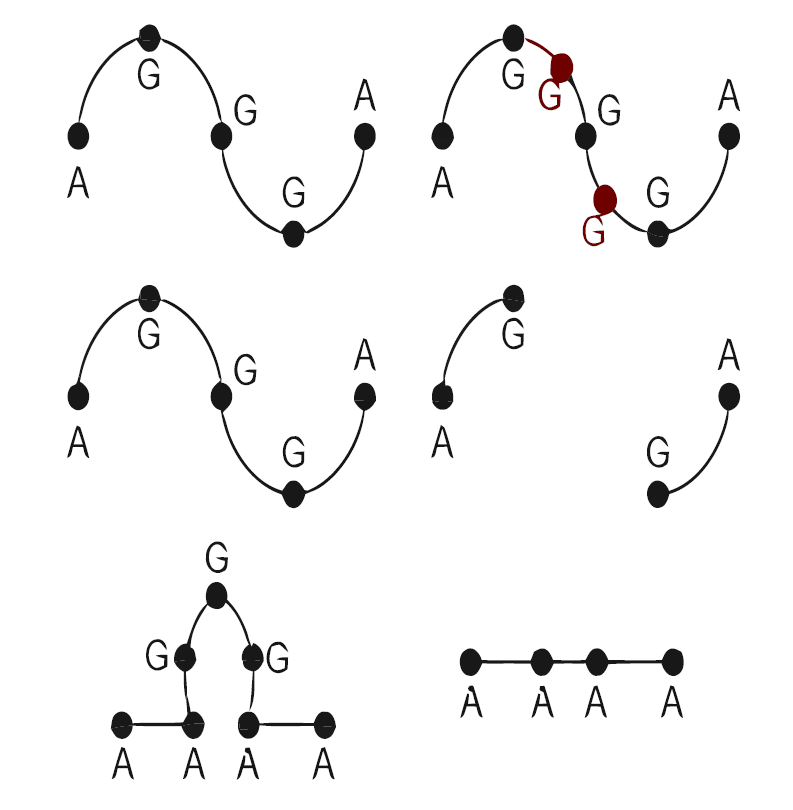
\includegraphics[width=\textwidth]{../img/aln-problems}
\caption{Problémy, ktoré môžu nasať v štruktúre pri vložení medzier do target alebo template časti zarovnania. Prvý riadok zobrazuje komplikácie pri pokuse vložiť nukleotidy do celistvej štruktúry (teda v zarovnaní boli pridané medzery do target sekvencie). Druhý riadok ukazuje opačný problém, a to vynechanie dvoch nukleotidov a roztrhnutie štruktúry (zodpovedá to vložením medzier to target sekvencie). Tretí riadok odpovedá rovnakej situácii ako druhý, ale odstránenie nukleotidov zo štruktúry nespôsobuje problém, pretože odstránené nukleotidy tvorili loop, ktorý môžeme bez problémov odobrať.}
\label{obr3.1:indels}
\end{figure}

Oba tieto problémy riešime tak, že nukleotidy v určitom okolí takýchto úsekov označíme za nekonzervované a budú dopredikované algoritmom FARFAR.
Taktiež označíme za nekonzervované tie nukleotidy, ktoré boli zarovnané na nezhodujúci sa typ nukleotidu. 


\indent V štvrtom kroku skopírujeme konzervované časti template štruktúry do predikovanej target štruktúry. Vzhľadom na to, že v zarovnaní môžu byť rôzne vložené medzery do target aj template sekvencie, musíme premapovať indexy nukleotidov z template štruktúry tak, aby odpovedali nukleotidom, na ktorých miesto sú vložené v target sekvencii. Toto urobíme jednoducho vďaka informáciám zo zarovnania. Takto získame target štruktúru s medzerami, ktoré potrebujeme dopredikovať.


\indent V piatom kroku identifikujeme dlhé nekonzervované úseky a vyčleníme ich následnu predikciu do samostatných behov algoritmu FARFAR. 
Prvým dôvodom je, že takto sa môže FARFAR zamerať iba na predikciu dlhého úseku, a tým znížime celkovú výpočetnú náročnosť. Takisto môžeme zmeniť jeho parametry, ako napríklad zvýšiť počet samplovaných modelov, prípade zvýšiť celkový čas predikcie. 
Ďalším dôvodom, prečo dopredikovanie nekonzervovaných úsekov takto delíme je, že algoritmus FARFAR sa nedokáže dobre vysporiadať s predikciami príliš dlhých štruktúr, aj keď je časť nukleotidov pevne daná. Z tohto dôvodu rozdeľujeme dlhé štruktúry na úseky dĺžky 300 nukleotidov na základe ich poradia v sekvencii. Takéto delenie spôsobuje ďalší problém - nukleotidy, ktoré sú od seba vzdialené v sekvencii môžu byť blízko pri sebe v terciárnej štruktúre. 
Naše riešenie teda vyberie tieto dlhé nekonzervované úseky spolu s okolitými nukleotidmi, ktoré ležia v guli so stredom určeným úsečkou spájajúcou posledný konzervovaný nukleotid pred nekonzervovaným úsekom s prvým konzervovaným nukleotidom za nekonzervovaným úsekom vzhľadom na ich poradie v sekvencii. Polomer tejto gule je určený experimentálne ako 0,75-násobok dĺžky úsečky, kedy by mala obsiahnuť všetky relevantné nukleotidy. \ref{obr3.2:sphere}

\begin{figure}%[p]\centering
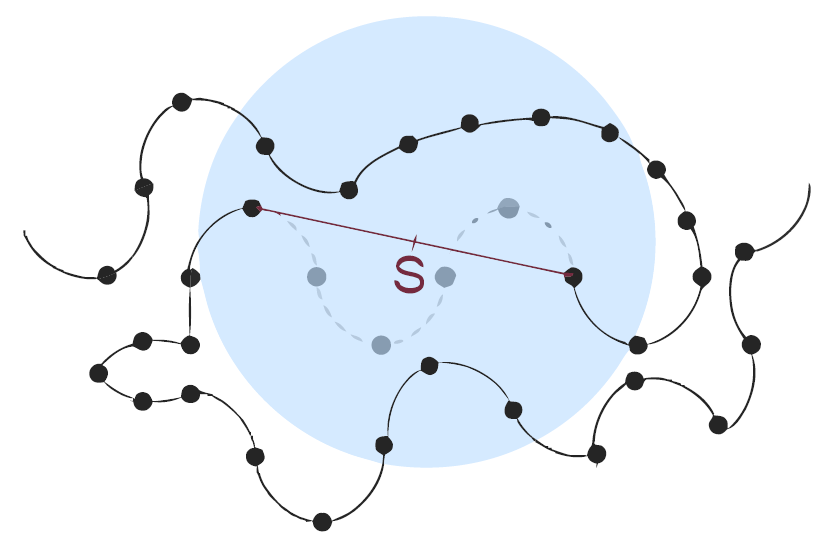
\includegraphics[width=\textwidth]{../img/sphere}
\caption{Schématické nakreslenie sféry so stredom v bode S, ktorý je stredom úsečky spájajúcej dva krajné konzervované nukleotidy medzery v štruktúre. Všetky nukleotidy, ktoré padnú do bledomodrej gule, budú použíte pri predikcii daného úseku.}
\label{obr3.2:sphere}
\end{figure}

\indent V šiestom kroku pripravíme vstupné dáta pre algoritmus FARFAR. To zahŕňa prípadné rozdelenie na úseky po 300 nukleotidov spomenuté v predchádzajúcom odstavci a prepísanie informácií o tom, ktoré nukleotidy sú pevne dané a ktoré treba dopredikovať do vstupného súboru. Takisto tu určíme parametre pre jednotlivé predikcie, ako napríklad počet vygenerovaných štruktúr.  


\indent
V siedmom kroku všetky takto pripravené časti predikcie spustíme a počkáme na výsledok. Toto je najpomalšia časť algoritmu, kedy FARFAR potrebuje čas minimálne pár hodín až niekoľko desiatok hodín, aby dokázal predikovať dlhšie nepredikované úseky. Tie sú napriek tomu najväčšou slabinou nášho algoritmu podľa výsledkov získaných v bakalárskej práci.


\indent V poslednom kroku najprv konvertujeme úseky z internej reprezentácie FARFARu do klasických pdb súborov a tie spojíme do výsledku.  


\section{Popis implementácie}
Algoritmus bol implementovaný prevažne v programovacom jazyku Python 2.7. s využitím knižnice BioPython, ktorá zjednodušuje prácu so štandardnými súbormi používanými v bioinformatike, ako napríklad pdb a fasta. Okrem toho používame bash scripty na manipuláciu so súbormi a spustenie predikcie vo FARFAR.


\indent Algoritmus bol rozdelený na tri časti. Prvá pozostávala zo spustenia predikcie dopredu pripravených dvojíc na lokálnom PC s operačným systémom Windows. To obsiahlo algoritmus  po siedmy krok, teda bola pipravená target štruktúra do stavu, kedy treba dopredikovať nekonzervované úseky algoritmom FARFAR. Následne boli takto pripravené vstupy pre FARFAR skopírované na servery organizácie Metacentrum používajúce operačný systém unixového typu s dávkovým spracovaním úloh, kde mohli bežať paralelne viaceré predikcie za pomoci FARFAR naraz. To je veľmi dôležité, pretože de novo predikcia nekonzervovaných úsekov bola najdlhšie trvajúca časť algoritmu a predikcia jednej štruktúry mohla obsahovať niekoľko takýchto de novo predikcií. Po skončení FARFAR predikcií nekonzervovaných úsekov boli výsledky skopírované späť na lokálny PC a tam boli v treťom kroku vyhodnotené výsledky. 


\indent Časová náročnosť celého algoritmu je závislá hlavne na nekonzevovaných úsekoch, ktoré treba predikovať. Časť predikcie po algoritmus FARFAR beží v rádoch desiatok sekúnd. Pre FARFAR sme okrem pár problémových predikcií používali obmedzenie predikcie časom 24 hodín, prípadne 100 štruktúr. Počet a kvalita kandidátskych štruktúr, ktoré za tento čas algoritmus stihne vygenerovať, záleží na počte nekonzervovaných úsekov, ich dĺžke (problematické sú hlavne dlhé nekonzervované úseky) a dĺžke celej predikovanej štruktúry včetne konzervovaných nukleotidov. Záverečné získanie výsledkov a porovnanie s experimentálne získanými štruktúrami prebieha opäť v rádoch desiatok sekúnd.


\section{Hlavné problémy algoritmu a jeho implementácie}
Najväčším problémom v našom algoritme, ktorý sme identifikovali na základe výsledkov bakalárskej práce, je predikcia dlhších nekonzervovaných úsekov \ref{obr3.3:badPredictedRegion}. Preto by sme potrebovali minimalizovať takéto úseky, prípadne pomôcť algoritmu FARFAR zmenšiť prehľadávaný priestror pri generovaní kandidátskych štruktúr. To by potom mohlo pomôcť rýchlosti predikcie kandidátskych štruktúr FARFAR-om a zlepšiť jeho presnosť.

\indent Takisto by sme chceli do väčšej miery automatizovať predikciu, presúnť ju celú na jedno prostredie a zbaviť sa tak nutnosti manuálneho kopírovania súborov. Okrem toho by sme ccheli predstaviť alternatívnu možnosť vstupných parametrov, kedy by nebolo treba určiť target aj template molekuly, ale stačilo by určiť target sekvenciu a algoritmus by sám našiel vhodnú štruktúru, ktorá by mohla slúžiť ako template. 

\begin{figure}%[p]\centering
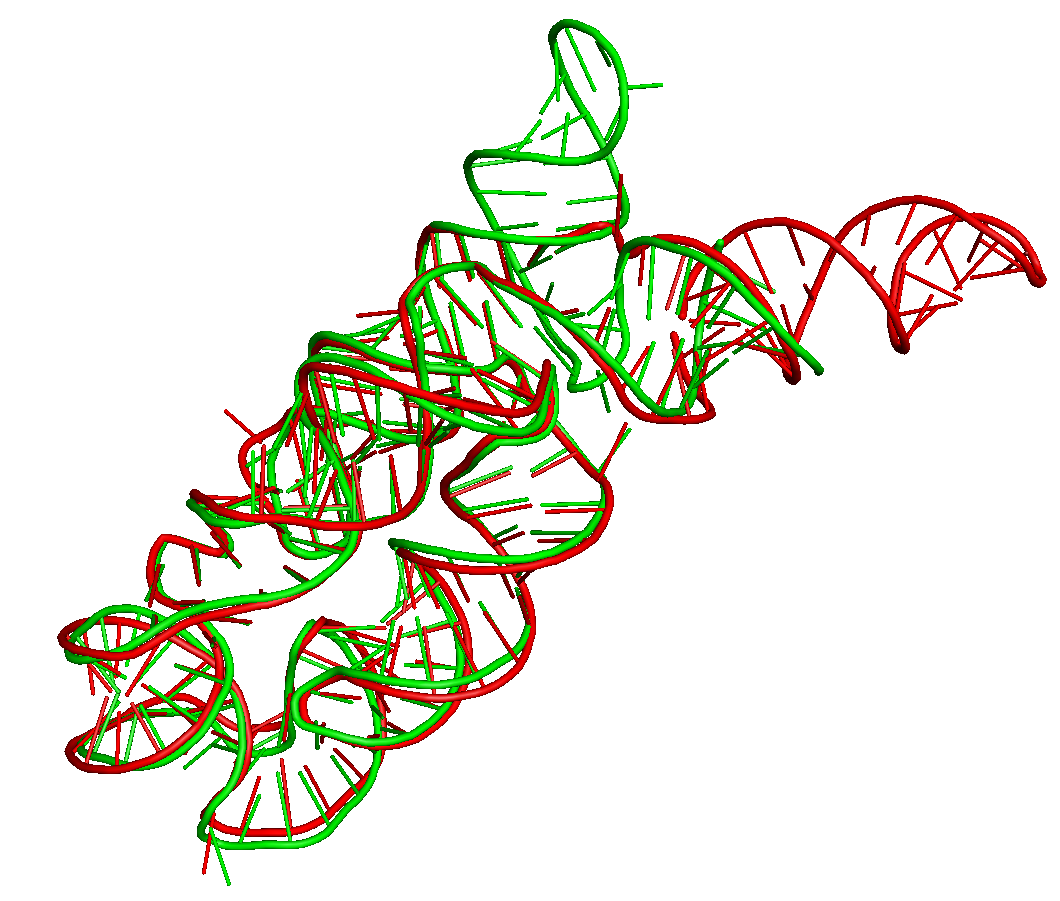
\includegraphics[width=\textwidth]{../img/badPredictedRegion}
\caption{Na obrázku vidíme zarovnanie experimenntálne získanej (3DIG) štruktúry a jej predikcie, napredikovanou našim algoritmom vytvoreným v bakalárskej práci. V pravej hornej časti obrázka vidíme, že algoritmu FARFAR sa nepodarilo správne napredikovať nekonzervovaný úsek.}
\label{obr3.3:badPredictedRegion}
\end{figure}
